\chapter{基礎概念}
\label{chap:concept}

\section{アドホックネットワーク}
アドホックネットワーク\cite{アドホック}とは,アクセスポイントを必要としない無線で接続できる端末のみで構成されたネットワークである.
直接電波が届き通信可能である場合には,始点端末から終点端末へ1ホップでパケット伝達が行われる.
電波が直接届かない場合には経由(マルチホップ)することで終点端末までパケットを伝達する.
端末の中継機能を利用してネットワークを構成しているので,アドホックネットワークには基地局インフラが不要である.
そのため、限られた領域内の簡易なネットワークの構築の手段として有効である.

以下の図では始点端末から終点端末まで直接繋がっていないが,他の端末を経由し4ホップで通信を行っている.

\begin{figure}[htbp]
\centering
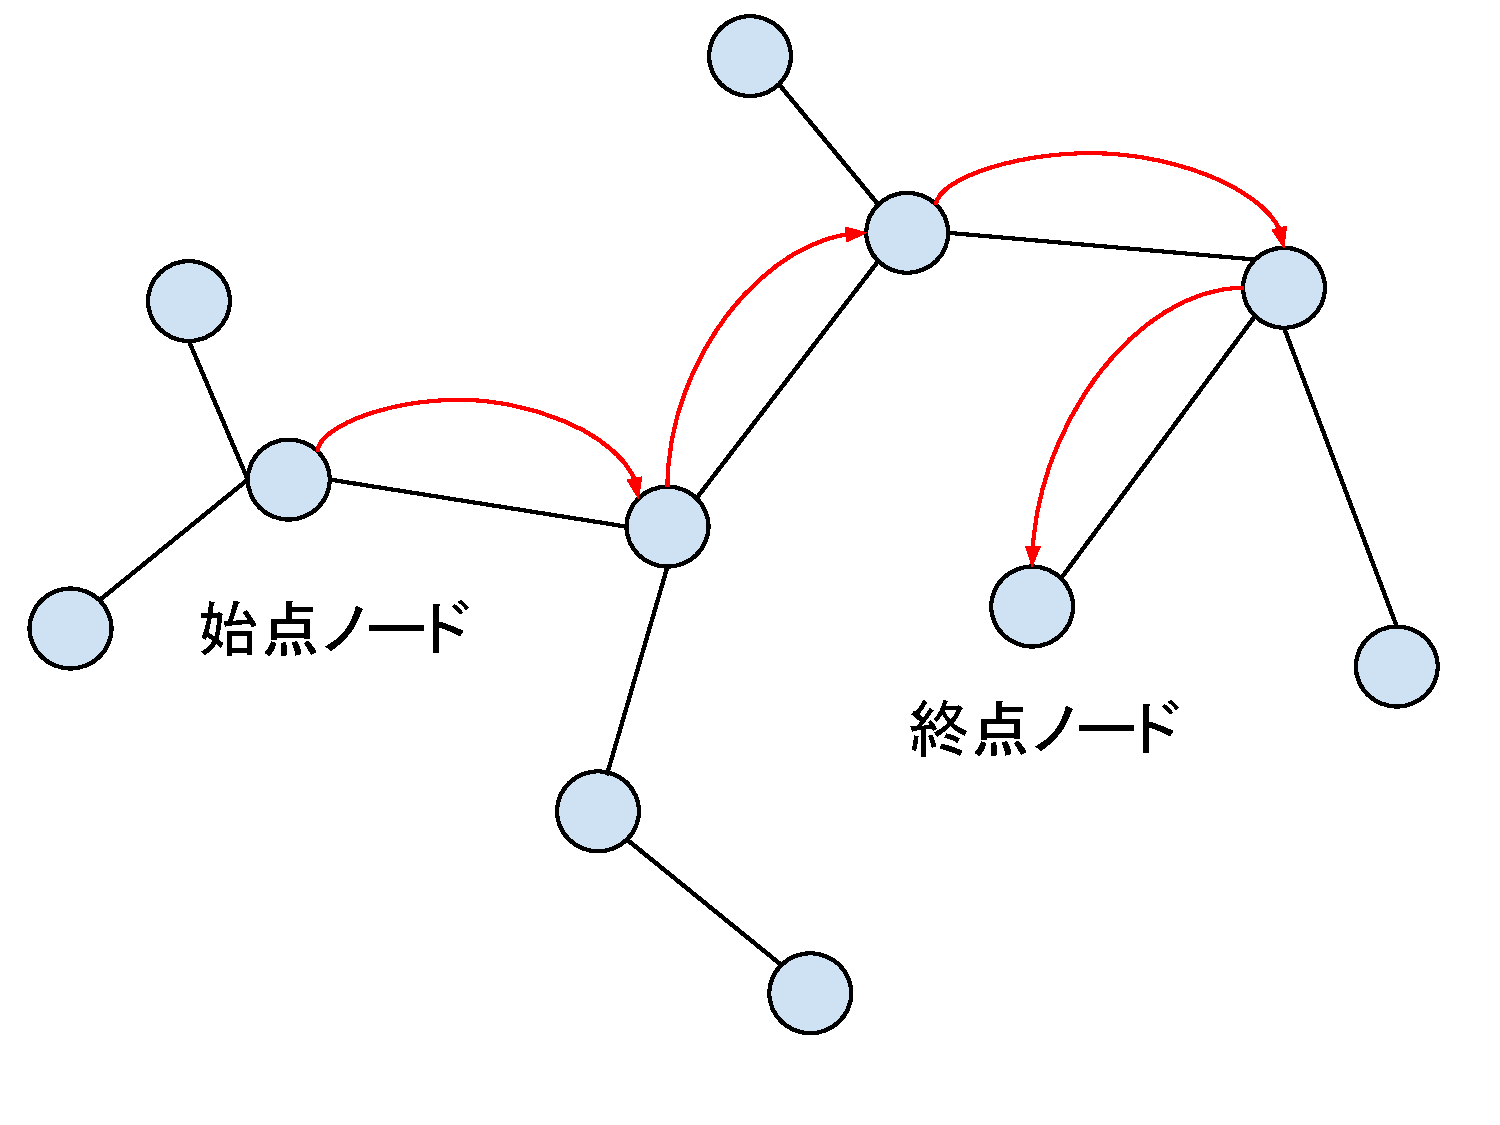
\includegraphics[width=10cm]{fig/ad-hoc.pdf}
\caption{アドホックネットワークの例}
\end{figure}

\section{AllJoyn}
AllJoyn\cite{allseen}\cite{スライド}はQualcommが開発したオープンソースプロジェクトである.
端末間通信を実現し,製品やアプリケーション間の相互運用を可能にするデバイス通信フレームワークを提供している.
QualcommはloT標準化団体であるAllSeenに参加しており,AllSeenが推進するloT規格はAllJoynをベースに設計されている.
OSI参照モデルのセッション層以上の規格であり,トランスポート層には依存しないというメリットがある.
そのため,Wi-FiやWi-Fi Direct,Bluetoothといった様々な通信規格を用いて開発することができる.
Android,iOS,OS X,Linux,Windows7など様々なOSに対応し,Java,C++,C,JavaScriptなどの言語で使用できる.
AllJoynは近傍デバイスの探索やP2Pネットワークへの接続,セキュリティなどの要素を提供しており,機器やOSに依存せず開発することができる.

\begin{figure}[htbp]
\centering
\includegraphics[width=10cm]{fig/AllJoyn_App.pdf}
\caption{AllJoynを用いたアプリケーションの例}
\end{figure}

\subsection{AllJoynアーキテクチャ}

AllJoynネットワークはAllJoynアプリケーションとAllJoynルーターから成る.
AllJoynアプリケーションはAllJoynルーターを通じて他のAllJoynアプリケーションやAllJoynルーターと通信を行う.
AllJoynアプリケーションは以下の要素から成る.

\begin{itemize}
\item AllJoyn App Cods
\item AllJoyn Service Frameworks Libraries
\item AllJoyn Core Library
\end{itemize}

\begin{figure}[htbp]
\centering
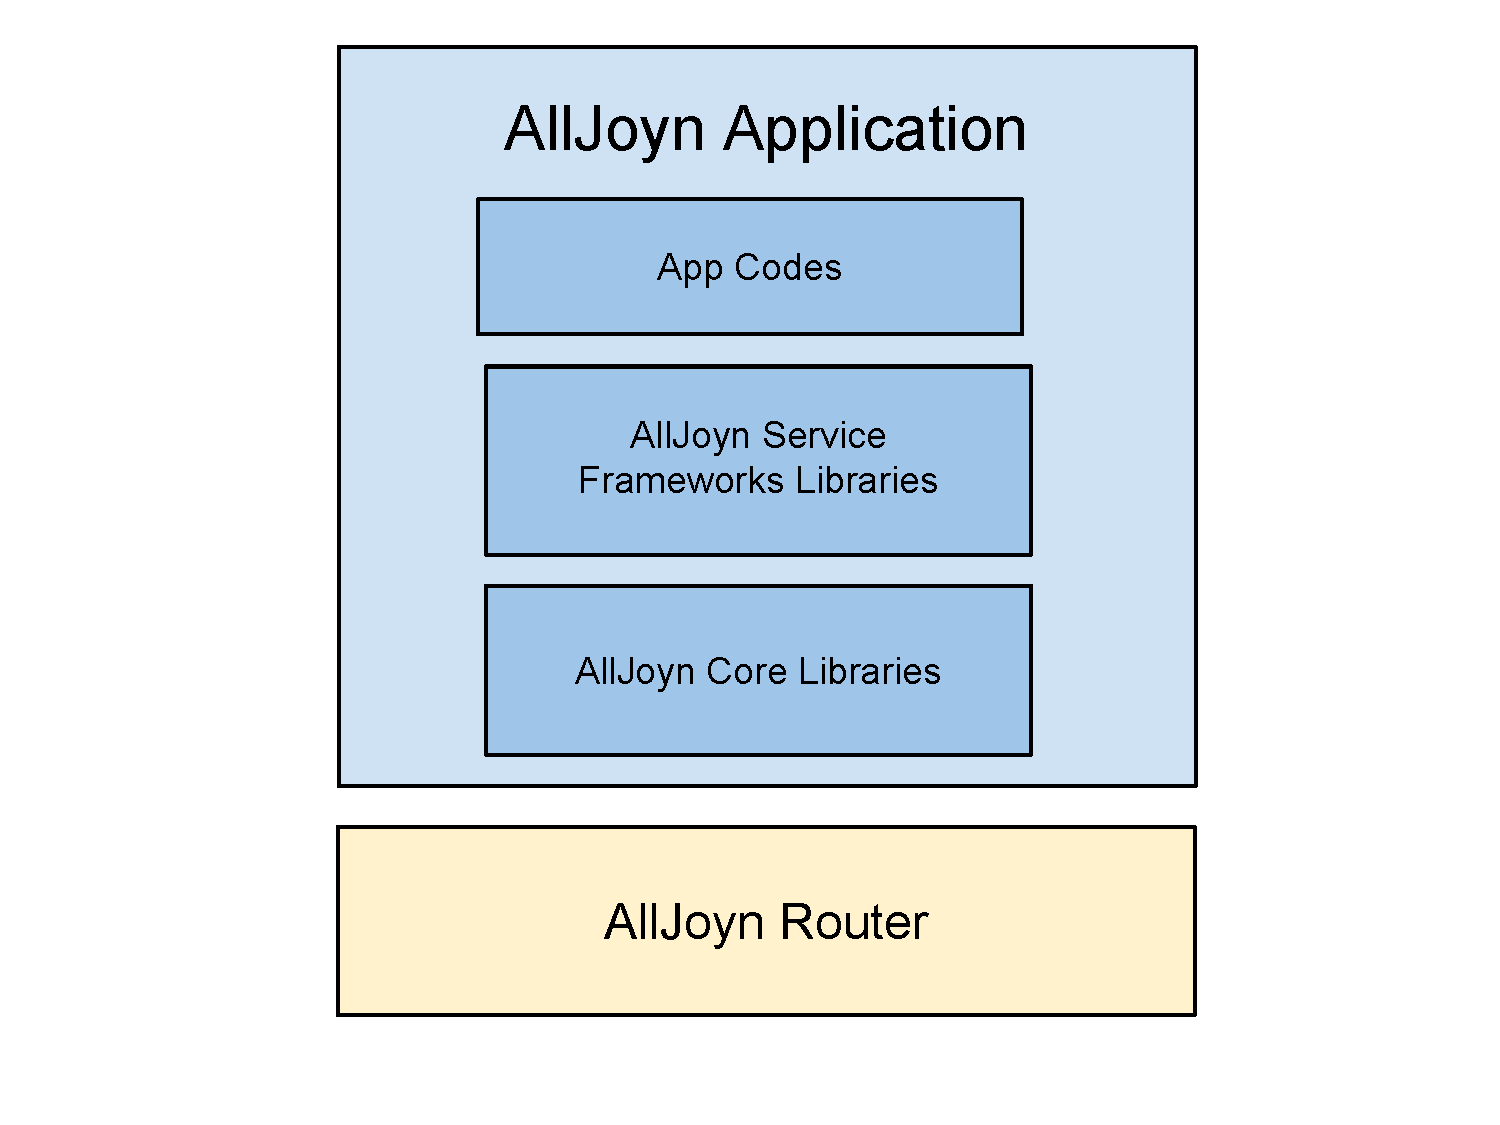
\includegraphics[width=10cm]{fig/AllJoyn.pdf}
\caption{AllJoynアーキテクチャの構成}
\end{figure}

\subsubsection{AllJoyn Core Library}
AllJoyn Core LibraryはAllJoynネットワークと通信するための最低限のAPIを提供する.
提供するAPIは以下の通りである.

\begin{itemize}
\item Advertisement \\
UDPパケットを用いてAllJoynサービスをブロードキャストする.
\item Discovery \\
AdvertisementされたAllJoynサービスを検索する.
\item Session creation \\
セッションの確立
\item Interface definition of methods, properties, and signals \\
メソッド,プロパティ,シグナルのインターフェース定義
\item Object creation and handling \\
オブジェクトの生成とハンドリング
\end{itemize}

\subsubsection{AllJoyn Service Framework Libraries}
AllJoyn Service Framework Librariesは,onboarding,notificatino,control panelなどのサービスを備えている.
Base Servicesとして以下の機能がある.

\begin{itemize}
\item Base Services
\begin{itemize}
\item Onbording \\
Wi-Fiネットワークへの接続をサポート
\item Configuration \\
端末の構成
\item Notificatinos \\
デバイスからの通知
\item Control Panel \\
UI widgetとリモート端末との通信
\end{itemize}
\end{itemize}

AllJoyn Service Framework Librariesを使うことで,アプリケーションや端末は互いにこれらのサービスを運用することができる.


\subsubsection{AllJoyn App Code}
AllJoyn App CodeはAllJoynアプリケーションのロジックである.
高レベルの機能を提供するAllJoyn Service Frameworksか,直接AllJoyn Core APIにアクセスできるAllJoyn Core Libraryのどちらかを用いてプログラミングされる.

\subsubsection{AllJoyn Router}
AllJoyn RouterはP2P Advertisement/Discovery,Connection ManagementといったAllJoynシステムの核となる機能を提供する.
メッセージはAllJoyn Routerを経由して他のアプリケーションに送信される.



\section{Bluetooth Low Energy}
Bluetooth Low Energy(BLE)\cite{BLE1}\cite{BLE2}近距離無線通信技術Bluetoothの拡張仕様の1つであり,Bluetooth4.0規格の一部として採用された.
一般的なBluetoohと同様に2.4GHz帯を使用し,データ転送速度は1Mbpsである.
非常に少ない消費電力で動作することができ,ボタン電池で数年動作すると言われている.

\section{iBeacon}
iBeacon\cite{iBeacon}\cite{iBeaconを使用してみよう}は,2013年にAppleが発表したBluetooth Low Energy(BLE)を利用した技術であり,発信機から発せられるビーコンを受信し,発信機の位置を特定・確認できる.
iOS7以降の端末(iPhone,iPad,およびiPod touch)やAndroid4.3以降の端末などで受信することができる.
iBeaconでは領域の出入りをチェックするリージョン監視やビーコンの情報を受信するレーシングを用いて位置や近接具合などを検知する.
ビーコンを受信したときに得られる情報には以下の6つがある.


\begin{comment}%コメントアウト

\begin{table}[htb]
\centering
\begin{tabular}{|l|l|}  \hline
proximityUUID & 識別子 \\ \hline
major & 識別子 \\  \hline
minor & 識別子 \\ \hline
proximity & ビーコンとの距離 \\ \hline
accuracy & 距離の精度 \\ \hline
RSSI & 受信強度 \\ \hline
\end{tabular}
\end{table}

\end{comment}

\begin{itemize}
\item proximity UUID:ビーコン識別子
\item major:ビーコン識別子
\item minor:ビーコン識別子
\item proximity:ビーコンとの距離
\item accuracy:距離の精度
\item rssi:受信強度
\end{itemize}

また,proximityは正確な距離を表すものではなく,以下の大まかな4つの値で得ることができる.

\begin{comment}%コメントアウト

\begin{table}[htb]
\centering
\begin{tabular}{|l|l|} \hline
Unknown & 検出不可 \\ \hline
Immediate & 至近距離 \\ \hline
Near & 近距離 \\ \hline
Far & 遠距離 \\ \hline
\end{tabular}
\end{table}

\end{comment}

\begin{itemize}
\item Unknown:検出不可
\item Immediate:至近距離
\item Near:近距離
\item Far:遠距離
\end{itemize}
